\documentclass[a4paper,10pt]{report}
\usepackage[utf8]{inputenc}
\usepackage{gensymb}
\usepackage{textcomp}
\usepackage{graphicx}

% Title Page
\title {\strong{Week 1 Update}}
\author{Rajat Saxena}

\begin{document}
\maketitle

\section{Survey of different motion capture technique using Kinect Camera}

\subsection{Adding Collision object for Human Body in Augmented Reality using Kinect}
\textbf{Research Paper:} Aitpayev, K.; Gaber, J., "Collision Avatar (CA): Adding collision objects for human body in augmented reality using Kinect," Application of Information and Communication Technologies (AICT), 2012 6th International Conference on, vol., no., pp.1,4, 17-19 Oct. 2012.
\subsubsection{Pros and Cons}
\begin{itemize}
 \item Easy to implement
 \item System not accurate enough
 \item problem with measurements of bone
\end{itemize}
\subsubsection{Illustrations}\newline\newline
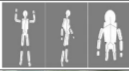
\includegraphics{./tech1.png}
% tech1.png: 0x0 pixel, 0dpi, 0.00x0.00 cm, bb=
\newline\newline

\subsection{Skeleton Animation motion data based on Kinect}
\textbf{Research Paper:} Xiaolong Tong; Pin Xu; Xing Yan, "Research on Skeleton Animation Motion Data Based on Kinect, "Computational Intelligence and Design (ISCID), 2012 Fifth International Symposium on , vol.2, no., pp.347,350, 28-29 Oct. 2012.
\subsubsection{Pros and Cons}
\begin{itemize}
 \item Creation of standard motion data files in real time
 \item reduces funding of implementation
 \item jitter present in data achieved for foot
 \item lack in optimization of motion data
\end{itemize}
\subsubsection{Illustrations}\newline\newline
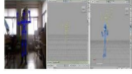
\includegraphics{./tech2.png}
% tech1.png: 0x0 pixel, 0dpi, 0.00x0.00 cm, bb=
\newline\newline


\subsection{Motion Capture and Reconstruction based on depth info using Kinect}
\textbf{Research Paper:} Ming Zeng; Zhengcun Liu; Qinghao Meng; Zhengbiao Bai; Haiyan Jia, "Motion capture and reconstruction based on depth information using Kinect," Image and Signal Processing (CISP), 2012 5th International Congress on , vol., no., pp.1381,1385, 16-18 Oct. 2012.
\subsubsection{Pros and Cons}
\begin{itemize}
 \item Fairly accurate reuslts obtained for real time 3D human body movements.
 \item Good fidelity and low latency of system
 \item no support for occlusion handling
\end{itemize}
\subsubsection{Illustrations}\newline\newline
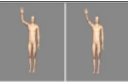
\includegraphics{./tech3.png}
% tech1.png: 0x0 pixel, 0dpi, 0.00x0.00 cm, bb=
\newline\newline


\subsection{Animation of 3D characters from single depth camera}
\textbf{Research Paper:} Mian Ma; Feng Xu; Yebin Liu, "Animation of 3D characters from single depth camera," 3D Imaging (IC3D), 2011 International Conference on, vol., no., pp.1,4, 7-8 Dec. 2011.
\subsubsection{Pros and Cons}
\begin{itemize}
 \item Noise and errors with joints position are removed
 \item Due to removal of noise good results are obtained
 \item The deformation models pose in not that similar to captured cahracter
 \item Skinning is not done properly
\end{itemize}
\subsubsection{Illustrations}\newline\newline
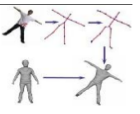
\includegraphics{./tech4.png}
% tech1.png: 0x0 pixel, 0dpi, 0.00x0.00 cm, bb=
\newline\newline


\subsection{Multiple user motion capture and system engineering}
\textbf{Research Paper:} Colvin, C.E.; Babcock, J.H.; Forrest, J.H.; Stuart, C.M.; Tonnemacher, M.J.; Wen-Shin Wang, "Multiple user motion capture and systems engineering," Systems and Information Engineering Design Symposium (SIEDS), 2011 IEEE , vol., no., pp.137,140, 29-29 April 2011.
\subsubsection{Pros and Cons}
\begin{itemize}
 \item Support for mapping hand gestures
 \item Reduces funding if implementation
 \item arm gestures not supported
\end{itemize}
\subsubsection{Illustrations}\newline\newline
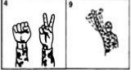
\includegraphics{./tech5.png}
% tech1.png: 0x0 pixel, 0dpi, 0.00x0.00 cm, bb=
\newline\newline


\subsection{Augmented Mirror: interactive AR system based on kinect}
\textbf{Research Paper:} Vera, Lucía, et al. "Augmented mirror: interactive augmented reality system based on kinect." Human-Computer Interaction–INTERACT 2011. Springer Berlin Heidelberg, 483-486. 2011.
\subsubsection{Pros and Cons}
\begin{itemize}
 \item Head orientaion, lip movements, facial expressions, and automatic gestures are handled
 \item Occlusion is handled
 \item Finger tracking is not supported
 \item use of too many devices makes system difficult to implement
\end{itemize}
\subsubsection{Illustrations}\newline\newline
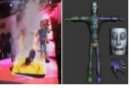
\includegraphics{./tech6.png}
% tech1.png: 0x0 pixel, 0dpi, 0.00x0.00 cm, bb=
\newline\newline


\subsection{Scanning 3D full human bodies using kinect}
\textbf{Research Paper:} Tong, Jing, et al. "Scanning 3d full human bodies using kinects." Visualization and Computer Graphics, IEEE Transactions on 18.4 (2012): 643-650.
\subsubsection{Pros and Cons}
\begin{itemize}
 \item inference phenomenon is handled using multiplekinect.
 \item complex occlusions are handled
 \item reduces funding of implementation
 \item algorithm is memory efficient
 \item quality of reconstructed model is still poor.
 \item misalignments still occur
 \item unnatural bending in arm areas
\end{itemize}
\subsubsection{Illustrations}\newline\newline
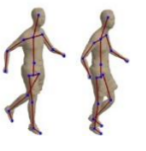
\includegraphics{./tech7.png}
% tech1.png: 0x0 pixel, 0dpi, 0.00x0.00 cm, bb=
\newline\newline


\subsection{Skeleton Tracking using kinect sensor and displaying in 3d virtual scene}
\textbf{Research Paper:} Chanjira Sinthanayothin, Nonlapas Wongwaen, Wisarut Bholsithi. Skeleton Tracking using Kinect Sensor & Displaying in 3D Virtual Scene. International Journal of Advancements in Computing Technology. IJACT: International Journal of Advancements in Computing Technology, Vol. 4, No.11, pp. 213 - 223, 2012.
\subsubsection{Pros and Cons}
\begin{itemize}
 \item Bone joint movements are detected in real time with correct position tracking
 \item No support for occlusion
\end{itemize}
\subsubsection{Illustrations}\newline\newline
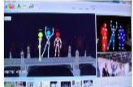
\includegraphics{./tech8.png}
% tech1.png: 0x0 pixel, 0dpi, 0.00x0.00 cm, bb=
\newline\newline


\subsection{Motion Capture by Kinect}
\textbf{Research Paper:} Karina Hadad de Souza, Rosilane Ribeiro da Mota. Motion Capture by inect. SBC - roceedings of SB ames, X SB ames – Bras lia – DF – Brazil, November 2nd - 4th, 2012.
\subsubsection{Pros and Cons}
\begin{itemize}
 \item Multiple kinect support for motion capture
 \item increase in precision of system
 \item occlusion handled with use of multiple kinect
 \item not good enough performance
 \item with use of multiple kinect data processing increase
\end{itemize}
\subsubsection{Illustrations}\newline\newline
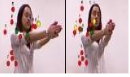
\includegraphics{./tech9.png}
% tech1.png: 0x0 pixel, 0dpi, 0.00x0.00 cm, bb=
\newline\newline


\subsection{Unsupervised Skeleton extraction and Motion Capture from Kinect video via 3D deformable matching}
\textbf{Research Paper:} Zhang, Quanshi, et al. "Unsupervised skeleton extraction and motion capture from 3D deformable matching." Neurocomputing 100 (2013): 170-182.
\subsubsection{Pros and Cons}
\begin{itemize}
 \item more robust approach than others
 \item good performance
 \item no support for occlusion in case when a person folds his hands together
\end{itemize}
\subsubsection{Illustrations}\newline\newline
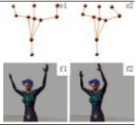
\includegraphics{./tech10.png}
% tech1.png: 0x0 pixel, 0dpi, 0.00x0.00 cm, bb=
\newline\newline


\subsection{Real time Physical modeling of character movements with microsoft kinect}
\textbf{Research Paper:} Shum, Hubert, and Edmond SL Ho. "Real-time physical modelling of character movements with microsoft kinect." Proceedings of the 18th ACM symposium on Virtual reality software and technology. ACM, 2012.
\subsubsection{Pros and Cons}
\begin{itemize}
 \item proposed algorithm is computationally efficient and can be applied to wide variety of interactive VR applications
 \item no support for occlusions and noise handling
\end{itemize}
\subsubsection{Illustrations}\newline\newline
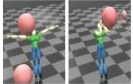
\includegraphics{./tech11.png}
% tech1.png: 0x0 pixel, 0dpi, 0.00x0.00 cm, bb=
\newline\newline



\section{Survey of body and skeleton tracking techniques}

\subsection{Optical Motion Capture}
\textbf{Research Paper:} Fern'ndez-Baena, Adso, Antonio Susin, and Xavier Lligadas. "Biomechanical validation of upper-body and lower-body joint movements of kinect motion capture data for rehabilitation treatments." Intelligent Networking and Collaborative Systems (INCoS), 2012 4th International Conference on.IEEE, 2012.
\subsubsection{Applications}
Biomechanical validation of upper body and lower body joint movements of kinect motion capture data for rehabilitation treatments
\subsubsection{Pros and Cons}
\begin{itemize}
 \item Reducing funding of implementation
 \item Comparison of Kinect motion capture with optical motion capture
 \item gives fairly good results
 \item lack of precision in system
 \item approximation of joints and bones not done
\end{itemize}
\subsubsection{Illustrations}\newline\newline
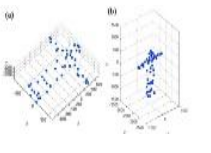
\includegraphics{./skeltrack1.png}
% skeltrack1.png: 0x0 pixel, 0dpi, 0.00x0.00 cm, bb=
\newline \newline

\subsection{Randomized decision forests}
\textbf{Research Paper:} J. Shotton, A. Fitzgibbon, M. Cook, T. Sharp, M. Finocchio, R. Moore, A. Kipman, and A. Blake. Real-time human pose recognition in parts from single depth images. In Computer Vision and Pattern Recognition (CVPR), 2011 IEEE Conference on, pages 1297 –1304, june 2011.
\subsubsection{Applications}
Real time human pose recognition in parts from single depth camera
\subsubsection{Pros and Cons}
\begin{itemize}
 \item quickly and accurately predicts 3D positions of body joints from single depth image, using no temporal information
 \item ability to run the classifier in parallel on each pixel on a GPU to increase the speed.
 \item using large and highly varied training dataset to estimate body parts invariants to pose, body shape, clothing, etc. to pose the relation between two adjacent parts.
\end{itemize}
\subsubsection{Illustrations}\newline\newline
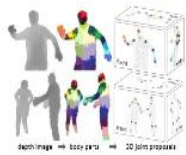
\includegraphics{./skeltrack2.png}
% skeltrack1.png: 0x0 pixel, 0dpi, 0.00x0.00 cm, bb=
\newline \newline

\subsection{Decentralized articulated object tracking. heirarchial articulated object tracking}
\textbf{Research Paper:} Qu, Wei, and Dan Schonfeld. "Real-time decentralized articulated motion analysis and object tracking from videos." Image Processing, IEEE Transactions on 16.8 (2007): 2129-2138.
\subsubsection{Applications}
Real time decentralized articulated motion analysis and object tracking from videos
\subsubsection{Pros and Cons}
\begin{itemize}
 \item fast and easy to implement
 \item results are not shown in case of self-occlusion due to the fact that it cannot pose relation between two adjacent parts.
\end{itemize}
\subsubsection{Illustrations}\newline\newline
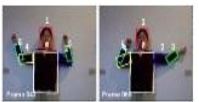
\includegraphics{./skeltrack3.png}
% skeltrack1.png: 0x0 pixel, 0dpi, 0.00x0.00 cm, bb=
\newline \newline

\subsection{position tracking based on a kalman filter, multiple particle-filter tracking based on 2D articulated motion}
\textbf{Research Paper:} del Rincón, Jesús Martínez, et al. "Tracking human position and lower body parts using Kalman and particle filters constrained by human biomechanics." Systems, Man, and Cybernetics, Part B: Cybernetics, IEEE Transactions on 41.1 (2011): 26-37.
\subsubsection{Applications}
Tracking human position and lower body parts using kalman and particle filter constrained by human biomechanics.
\subsubsection{Pros and Cons}
\begin{itemize}
 \item bipedal motion is handled without any constraints
 \item occlusion is seen in case of pivot joints.
\end{itemize}
\subsubsection{Illustrations}\newline\newline
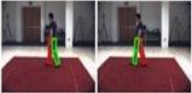
\includegraphics{./skeltrack4.png}
% skeltrack1.png: 0x0 pixel, 0dpi, 0.00x0.00 cm, bb=
\newline \newline

\subsection{Gaussian process annealed particle filter}
\textbf{Research Paper:} Raskin, Leonid, Michael Rudzsky, and Ehud Rivlin. "Dimensionality reduction using a Gaussian Process Annealed Particle Filter for tracking and classification of articulated body motions." Computer Vision and Image Understanding 115.4 (2011): 503-519.
\subsubsection{Applications}
Gaussian process annealed particle filter for tracking and classification of articulated body motions.
\subsubsection{Pros and Cons}
\begin{itemize}
 \item robust than heirarchial annealed particle filter.
 \item less errors
 \item in case of hugging motion classification fails.
 \item cross validation is needed to classify ambiguous types of motion
\end{itemize}
\subsubsection{Illustrations}\newline\newline
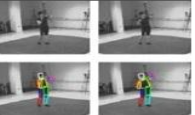
\includegraphics{./skeltrack5.png}
% skeltrack1.png: 0x0 pixel, 0dpi, 0.00x0.00 cm, bb=
\newline \newline

\subsection{Recursive Bayesian Tracking for articulated objects}
\textbf{Research Paper:} Bernier, Olivier, Pascal Cheung-Mon-Chan, and Arnaud Bouguet. "Fast nonparametric belief propagation for real-time stereo articulated body tracking." Computer Vision and Image Understanding 113.1 (2009): 29-47.
\subsubsection{Applications}
fast non parametric belief propogation for real-time the tri axis internal/ magnetic sensors package
\subsubsection{Pros and Cons}
\begin{itemize}
 \item good results shown arm movements to various human positions
 \item slow processing rates.
\end{itemize}
\subsubsection{Illustrations}\newline\newline
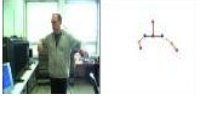
\includegraphics{./skeltrack6.png}
% skeltrack1.png: 0x0 pixel, 0dpi, 0.00x0.00 cm, bb=
\newline \newline

\subsection{Kalman based fusion algorithm}
\textbf{Research Paper:} Zhu, Rong, and Zhaoying Zhou. "A real-time articulated human motion tracking using tri-axis inertial/magnetic sensors package." Neural Systems and Rehabilitation Engineering, IEEE Transactions on 12.2 (2004): 295-302.
\subsubsection{Applications}
Real time decentralized articulated motion analysis and object tracking from videos
\subsubsection{Pros and Cons}
\begin{itemize}
 \item accurate tracking is achieved by use of kalan filter to eliminate
 \item time lag is generated du to kalman filter.
\end{itemize}
\subsubsection{Illustrations}\newline\newline
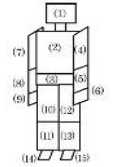
\includegraphics{./skeltrack7.png}
% skeltrack1.png: 0x0 pixel, 0dpi, 0.00x0.00 cm, bb=
\newline \newline

\subsection{Grid based belief propogation algorithm, data-driven markov chain monte carlo}
\textbf{Research Paper:} Lee, Mun Wai, and Ramakant Nevatia. "Human pose tracking in monocular sequence using multilevel structured models." Pattern Analysis and Machine Intelligence, IEEE Transactions on 31.1 (2009): 27-38.
\subsubsection{Applications}
human pose tracking in monocular sequence using multilevel structured models
\subsubsection{Pros and Cons}
\begin{itemize}
 \item less position error due to full pose inference
 \item longer processing time for rendering hence not suitable for real time application
\end{itemize}
\subsubsection{Illustrations}\newline\newline
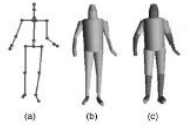
\includegraphics{./skeltrack8.png}
% skeltrack1.png: 0x0 pixel, 0dpi, 0.00x0.00 cm, bb=
\newline \newline

\subsection{Annealed Particle Filter, particle filter, factored-state heirarchial hidden markov model}
\textbf{Research Paper:} Peursum, Patrick, Svetha Venkatesh, and Geoff West. "A study on smoothing for particle-filtered 3d human body tracking." International Journal of Computer Vision 87.1-2 (2010): 53-74.
\subsubsection{Applications}
Smoothing for particle filtered 3d human body tracking
\subsubsection{Pros and Cons}
\begin{itemize}
 \item smoothed inference techniques are implemented
 \item occlusion and poor segmentation is handled by heirarchial hidden markov model
 \item tracking results are not so accurate
 \item smoothing does not improve body tracking accuracy
 \item processing time is increased due to smoothing
\end{itemize}
\subsubsection{Illustrations}\newline\newline
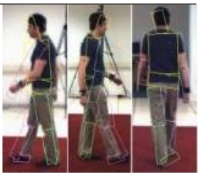
\includegraphics{./skeltrack9.png}
% skeltrack1.png: 0x0 pixel, 0dpi, 0.00x0.00 cm, bb=
\newline \newline

\subsection{Variable length markov models, monte-carlo bayesian frame-work}
\textbf{Research Paper:} Caillette, Fabrice, Aphrodite Galata, and Toby Howard. "Real-time 3-D human body tracking using learnt models of behaviour." Computer Vision and Image Understanding 109.2 (2008): 112-125.
\subsubsection{Applications}
real time 3d human body tracking using learnt models of behavior
\subsubsection{Pros and Cons}
\begin{itemize}
 \item capable of handling fast and complex motions in real time
 \item body movements are captured while elimination jitters
 \item algorithm is robust and efficient
 \item simultaneously tracking of multiple subjects has not yet been fully investigated
 \item dimensionality reduction is needed on learning cluster
\end{itemize}
\subsubsection{Illustrations}\newline\newline
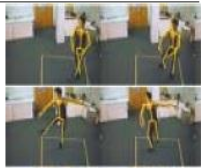
\includegraphics{./skeltrack10.png}
% skeltrack1.png: 0x0 pixel, 0dpi, 0.00x0.00 cm, bb=
\newline \newline


\section{Survey of different depth cameras with their specifications}

  \subsubsection{Kinect Camera}
  \textbf{Illustration}\newline
  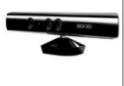
\includegraphics{./kinect.png}
% kinect.png: 0x0 pixel, 0dpi, 0.00x0.00 cm, bb=
\newline
  \textbf{Viewing Angle} 43\textdegree vertical by 57\textdegree horizontal\newline
  \textbf{Device Range} Minimum 0.8 meter to maximum 4 meter\newline
  \textbf{Frame Rate} 12 and 30 frames per second\newline
  \textbf{Rsolution} 1280 x 9960 resolution \newline
  \textbf{IR Camera} Yes\newline
  \textbf{Microphone array} Yes\newline
  \textbf{OS Support} Windows\newline
  \textbf{Comments}
  \begin{itemize}
  \item widely  used for gaming and application development                                                                                                                                                                                                                                                                                                                                                                                                                                                                                                                                                                                                                                                                                                                                                                                                                                                                                                                                                                                                                                                                                                                                                                                                                                                                                                                                                                                                                                                                                                                                                                                                                                                                                                                                                                                                                                                                                                                                                                                                                                                                                                                                                                                                                                                                                                                                                                                                                                                                                                                                                                                                                                                                                                                                                                                                                                                                                                                                                                                                                                                                                                                                                                                                                                                                                                                                                                                                                                                                                                                                                                                                                                                                                                                                                                                                                                                                                                                                                                                                                                                                                                                                                                                                     
  \item drivers are made available from Microsoft as well as third party drivers are also available
  \end{itemize}

\subsubsection{Sony Playstation Eye}
\textbf{Illustration}\newline
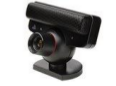
\includegraphics{./sony.png}
% sony.png: 0x0 pixel, 0dpi, 0.00x0.00 cm, bb=
\newline
\textbf{Viewing Angle} 56\textdegree to 75\textdegree field of view\newline
\textbf{Device Range} Minimum 0.3 meter\newline
\textbf{Frame Rate} 75 and 187 frames per second\newline
\textbf{Rsolution} 380 x 240 resolution at 12 FPS or a 640 x 480 resolution at 75 FPS \newline
\textbf{IR Camera} No\newline
\textbf{Microphone array} Yes\newline
\textbf{OS Support} Windows, Mac OS, Linux \newline
\textbf{Comments}
\begin{itemize}
 \item drivers are still not available from Sony
 \item play station playing experience is enhanced
\end{itemize}

\subsubsection{Prime Sense Sensor}
\textbf{Illustration}\newline
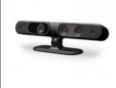
\includegraphics{./prime_sensor.png}
% prime_sensor.png: 0x0 pixel, 0dpi, 0.00x0.00 cm, bb=
\newline
\textbf{Viewing Angle} 57.5\textdegree to 45\textdegree field of view\newline
\textbf{Device Range} Minimum 0.8 meter to maximum 3.5 meter\newline
\textbf{Frame Rate} 60 frames per second (FPS)\newline
\textbf{Rsolution} 640 x 480 resolution \newline
\textbf{IR Camera} Yes\newline
\textbf{Microphone array} Yes\newline
\textbf{OS Support} Windows, Linux\newline
\textbf{Comments}
\begin{itemize}
 \item best depth performance
 \item low power consumption
 \item OpenNI compatible
\end{itemize}

\subsubsection{Intel's Creative Camera}
\textbf{Illustration}\newline
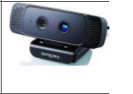
\includegraphics{./intel.png}
% intel.png: 0x0 pixel, 0dpi, 0.00x0.00 cm, bb=
\newline
\textbf{Viewing Angle} 73\textdegree field of view (diagonal)\newline
\textbf{Device Range} Minimum 0.15 meter to maximum 0.99 meter\newline
\textbf{Frame Rate} 30 frames per second (FPS)\newline
\textbf{Rsolution} 1280 x 720 resolution \newline
\textbf{IR Camera} Yes\newline
\textbf{Microphone array} Yes\newline
\textbf{OS Support} Windows\newline
\textbf{Comments}
\begin{itemize}
 \item very limited range
 \item portable camera with HD support
 \item drivers are made availablem from Intel
\end{itemize}



\section{Comparison of Natural User Interfaces(NUI) libraries}

\subsection{Microsoft Kinect SDK}
\subsubsection{Pros}
\begin{itemize}
 \item Easy to install, fairly widespread
 \item new version supports skeleton tracking
 \item able to grab full 1280x960 resolution of camera
 \item predictive tracking of joints
 \item skeleton recognition is done very fast
 \item joint occlusions handled
 \item description of sdk architecture and documentation for the APIs
\end{itemize}
\subsubsection{Cons}
\begin{itemize}
 \item support for windows only
 \item limited language support, only for c/c++ and c#
 \item higher processing power
\end{itemize}

\subsection{OpenNI/Nite}
\subsubsection{Pros}
\begin{itemize}
 \item very poppular, ready to use methods
 \item supports skeleton tracking
 \item available for most languages
 \item any OS compatible
\end{itemize}
\subsubsection{Cons}
\begin{itemize}
 \item difficult to install
 \item calibration pose is reqiored
 \item no predictive tracking
 \item joint occlusion not handled properly
 \item gets confused with very fast movements
\end{itemize}

\subsection{Libfreenect}
\subsubsection{Pros}
\begin{itemize}
 \item Support for several applications
 \item any OS compatible
 \item available for most languages
\end{itemize}
\subsubsection{Cons}
\begin{itemize}
 \item difficult to install
 \item no skeleton tracking
\end{itemize}

\subsection{CL NUI}
\subsubsection{Pros}
\begin{itemize}
 \item can capture wide range of body movements
 \item camera noise can be filtered
\end{itemize}
\subsubsection{Cons}
\begin{itemize}
 \item cannot perform motion prediction
 \item no support for occlusion handling
\end{itemize}

\subsection{Evoluce SDK}
\subsubsection{Pros}
\begin{itemize}
 \item supports various gesture recognition methods
 \item easy to install
 \item supports skeleton tracking
\end{itemize}
\subsubsection{Cons}
\begin{itemize}
 \item only for windows 7
 \item calibration pose is required
 \item limited language support, only for C/C++ and C#.
\end{itemize}

\subsection{Delicode NImate}
\subsubsection{Pros}
\begin{itemize}
 \item quite fast
 \item supports skeleton tracking
 \item does not require camera calibration
\end{itemize}
\subsubsection{Cons}
\begin{itemize}
 \item skeleton tracking not done properly
 \item only for windows
\end{itemize}

\end{document}          
